\documentclass[10pt,twocolumn]{article}
\usepackage[T1]{fontenc}
\usepackage{lmodern,microtype,amsmath,graphicx,booktabs}
\usepackage[a4paper,margin=17mm,columnsep=7mm]{geometry}
\usepackage[font=small,labelfont=normalfont]{caption}
\usepackage[hidelinks]{hyperref}
\raggedbottom
\hypersetup{pdftitle={Agent-guided model exploration for CYP inhibition prediction},pdfauthor={Somerra}}
\setlength{\parindent}{1em}
\setlength{\parskip}{0pt}
\setlength{\textfloatsep}{9pt}
\setlength{\intextsep}{8pt}
\setlength{\abovecaptionskip}{4pt}
\title{\vspace{-12mm}\Large Agent-guided model exploration for CYP inhibition prediction}
\author{\normalsize Somerra}
\date{\small OpenADMET CYP Challenge\quad |\quad 4 November 2026\vspace{-5mm}}
\begin{document}
\maketitle
\begin{abstract}
We used research agents to compare molecular representations, auxiliary assays,
architectures, and ensembles for CYP inhibition prediction. An audited sequence
of 540 scored evaluations covered 433 within-campaign recipe groups and
represented 1,543 model fits. A hit-expansion evaluation approximated the
challenge's selection of analogs around potent training compounds. Improvements
on this split did not consistently transfer to the leaderboard. The final
candidate combines 40 Chemprop networks. This study illustrates how agents can broaden
and document experimental exploration, while also exposing the limits of
adaptive internal evaluation.
\end{abstract}

\section{Research process and scope}
Humans set the objectives and constraints; agents maintained an idea queue,
implemented experiments, interpreted results, and revised the queue. Scripts
dispatched training jobs and monitored execution. This separation allowed
long-running searches without continuous model interaction. Negative results
informed subsequent experiments rather than disappearing from the record.

The audit counts completed scored evaluations, including controls and repeated
initialization seeds (Fig.~\ref{fig:volume}). Recipe groups are deduplicated
within campaigns, not across the entire project. Fit counts expand each
evaluation's folds or rotations. Failed or incomplete jobs, smoke tests,
duplicate records, submission refits, and calibration-only processing are
excluded. Separate foundation-model and specialist studies fall outside this
total. These numbers measure exploration, not independent discoveries. We did
not compare productivity against a human-only research team.

\begin{figure}[ht]
\centering
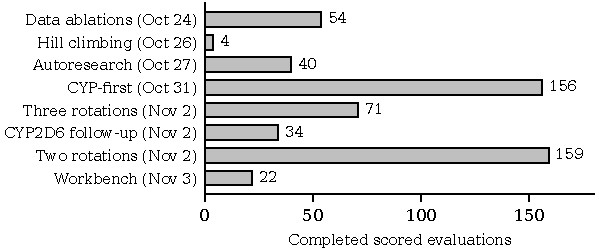
\includegraphics[width=\columnwidth]{figures/research-volume.pdf}
\caption{Completed scored evaluations by campaign. The final 22 configurations
account for 440 model fits; evaluations therefore differ in computational cost.}
\label{fig:volume}
\end{figure}

\section{Molecular representations}
Morgan fingerprints encode fixed local two-dimensional substructures and
provide inexpensive inputs for tree and linear controls. Chemprop models learn
atom--bond message-passing representations from assay labels, with shared
encoders supporting auxiliary outputs. CheMeleon~\cite{chemeleon} adds a
descriptor-pretrained graph encoder; comparisons included frozen features,
tree and neural heads, and encoder adaptation. A SMILES transformer instead
learns from molecular strings. Its completed pilot did not outperform its
graph reference.

Atom-JEPA~\cite{atom} tested a different source of information: atom types and
three-dimensional coordinates. We generated conformers with RDKit
ETKDGv3/MMFF94 and compared 256-dimensional scalar features with
768-dimensional features incorporating higher-order invariant norms. Further
experiments varied scaling, heads, task weights, losses, and conformer
sampling. Rotation and translation checks, together with checkpoint replay,
tested numerical consistency. Multi-conformer training and prediction
averaging were treated separately; an averaging gain alone does not establish
a benefit from geometry. Atom-JEPA improved one CYP1A2 development comparison
but did not show a consistent advantage across evaluations. Mol-JEPA is
retained in the historical record but excluded from the corporate-use
candidate set. Neither JEPA model contributes to the final predictor.

\section{Evaluation under hit expansion}
The official challenge expanded the top 25 training hits for CYP1A2, CYP2C9,
and CYP3A4 into close analogs; CYP2D6 did not nominate hits~\cite{challenge}.
Our analogous split reserved half of standardized official parents as a
training seed pool (random seed 42). Only seed-pool labels selected hits, using
pIC$_{50}\geq5$ for the three nominating CYPs. Structures alone selected up to
ten analogs per hit from the other half, using 2,048-bit Morgan fingerprints
(radius 2) and Tanimoto similarity $\geq0.50$. We used a larger potent-hit bank
than the official top-25 quota to improve coverage.

Overlapping nomination families remained together when balanced into groups
A and B; neither assay values nor assay availability determined assignment.
All bank and official blind parents were excluded from every training source,
including standardized aliases. Potent seed hits remained eligible for training.
Training stayed fixed while A and B exchanged checkpoint-validation and scoring
roles (Fig.~\ref{fig:split}). Each scored compound therefore used a fresh fit
whose checkpoint was selected on the other group.

\begin{figure}[ht]
\centering
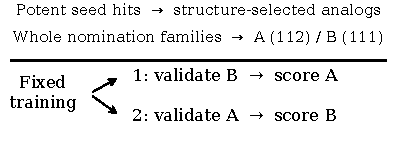
\includegraphics[width=\columnwidth]{figures/hit-expansion-logic.pdf}
\caption{Two-rotation evaluation. The 223-parent analog bank is excluded from
the fixed training set of 32,686 records. Validation selects checkpoints;
scoring predictions are pooled across rotations.}
\label{fig:split}
\end{figure}

The bank contains only 42, 38, 42, and 156 measured labels for CYP1A2, CYP2C9,
CYP2D6, and CYP3A4, respectively. Reducing three rotations to two enlarges each
scoring group without adding observations. Comparisons use the same saved
split and matched initialization seeds; scores from the three-rotation split
are not directly compared. Repeated adaptive use makes these development
results, not independent test estimates.

\begin{figure}[ht]
\centering
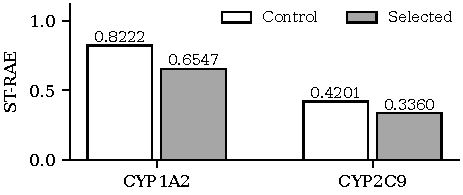
\includegraphics[width=\columnwidth]{figures/hit-expansion-progress.pdf}
\caption{Matched hit-expansion development results after averaging raw
predictions over three seeds. Lower ST-RAE is better. Both selected variants
improved error in both rotations; CYP2D6 and CYP3A4 controls were retained.}
\label{fig:progress}
\end{figure}

\newpage
The CYP1A2 variant combined Atom-JEPA, a Huber head, task weighting, a lower
learning rate, and removal of qHTS auxiliaries. The CYP2C9 variant removed TDI
auxiliaries. CYP1A2 subsequently worsened on Workbench and the official
leaderboard, motivating a return to Workbench-led selection. Structural
resemblance did not guarantee transfer. The final ensemble has not been
freshly evaluated on the analog bank.

\newpage
\section{Final ensemble}
Official challenge, ChEMBL, and Veith/PubChem measurements are represented as
separate masked outputs~\cite{workbench,data}. Two freshly trained Chemprop
configurations each use four task bundles and five preserved Workbench
scaffold folds, giving 40 networks. The two configurations use depth 5/7,
width 700, dropout 0.10/0.05, auxiliary weight 0.30/0.60, and peak learning
rate 0.001/0.0005. Both use two width-300 head layers, weighted MAE, batch
size 64, training-only target scaling, and early stopping (400 epochs
maximum; patience 40). Blind and fold-validation parents are excluded from
training. Predictions are averaged equally over folds, applicable bundles,
and configurations in raw pIC$_{50}$ units.

Matched Workbench macro out-of-fold (OOF) ST-RAE improved from 0.63943 to
0.61159 (4.35\%), with lower error and higher Spearman correlation for all
four endpoints. These checkpoint- and ensemble-selected results are
development evidence, distinct from Fig.~\ref{fig:progress}.

\begin{center}
\small
\begin{tabular}{lrr}
\toprule
Endpoint & Control & Final ensemble \\
\midrule
CYP1A2 & 0.75764 & 0.72200 \\
CYP2C9 & 0.55774 & 0.51686 \\
CYP2D6 & 0.82446 & 0.81078 \\
CYP3A4 & 0.41786 & 0.39672 \\
\bottomrule
\end{tabular}
\end{center}

After raw averaging, predictions were rescaled using the historical
Workbench leaderboard-informed transform~\cite{workbench}. The accompanying
\href{https://github.com/Somerra/somerra-openadmet-cyp/blob/main/report/reproducibility.md}{reproducibility note}
records the exact postprocessing and its provenance.

The candidate uses no proprietary training data or external
prediction files. Its 750-row CSV passed local validation; no official score
for this candidate is claimed. Code, report source, and aggregate figure data
are provided in the accompanying repository; trained checkpoints are not
included.

\begingroup
\small
\setlength{\parskip}{0pt}
\begin{thebibliography}{5}
\setlength{\itemsep}{0pt}
\bibitem{chemeleon} CheMeleon. \href{https://arxiv.org/abs/2506.15792}{arXiv:2506.15792}.
\bibitem{atom} Atom-JEPA. \href{https://huggingface.co/atom-jepa/atom-jepa}{Molecular checkpoint and model card}.
\bibitem{challenge} OpenADMET. \href{https://openadmet.ghost.io/halfway-through-the-openadmet-cyp-challenge/}{CYP challenge design and interim results}, 2026.
\bibitem{workbench} ADMET Workbench. \href{https://supercowpowers.github.io/workbench/blogs/cyp_challenge/}{CYP challenge working notes}.
\bibitem{data} OpenADMET. \href{https://huggingface.co/datasets/openadmet/cyp-challenge-train-test}{CYP challenge training and test dataset}.
\end{thebibliography}
\endgroup
\end{document}
